
\textbf{\underline{Вторая глава}} раскрывает решения трех оптимизационных задач, связанных с оптимизацией конструкции робота.

\textbf{Первая задача:} оптимизировать количество ног у объекта исследования на основе критериев \pic{fig:opti_criteria}. 

\begin{figure}[H]
    \begin{subfigure}{0.49\textwidth}
        \centering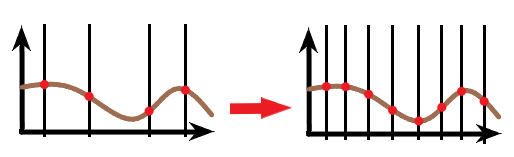
\includegraphics[height=6cm,width=1\textwidth,keepaspectratio]{f1.png}
        \caption{При увеличении количества ног увеличивается детализация картографируемой поверхности}
        \label{fig:f1.png}
    \end{subfigure}
    \begin{subfigure}{0.49\textwidth}
        \centering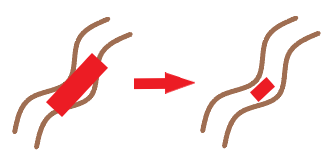
\includegraphics[height=6cm,width=1\textwidth,keepaspectratio]{f2.png}
        \caption{При увеличении количества ног, корпус робота увеличивается и он не может пройти часть препятствий}
        \label{fig:f2.png}
    \end{subfigure}

    \hfill
    \begin{subfigure}{\textwidth}
        \centering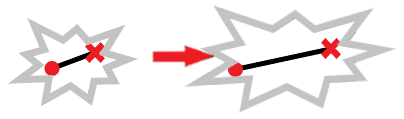
\includegraphics[height=2cm,width=1\textwidth,keepaspectratio]{f3.png}
        \caption{При увеличении количества ног увеличивается проходимость системы}
        \label{fig:f3.png}
    \end{subfigure}
    \hfill

\caption{Критерии оптимизации конструкции робота}
\label{fig:opti_criteria}
\end{figure}

ем больше ног имеет робот, тем более детально он может «ощупать» поверхность за один проход. В тоже время, при достаточно большом количестве ног дальнейшее увеличение их количества уже не будет давать значительного увеличения получаемой информации. С другой стороны, увеличение количества ног означает удлинение корпуса робота, что ухудшает его проходимость в узких проходах. Увеличение количества ног и связанное с этим удлинение корпуса также способствуют увеличению профильной проходимости робота, поскольку длинный робот с большим количеством ног легче преодолевает препятствия типа ям или траншей. Проходимость оценивается по длине пройденного роботом пути за заданное время при перемещении по заданной поверхности. Таким образом, сформулированы три критерия: детализация построенной карты, проходимость в узких проходах и профильная проходимость робота, которые зависят от количества ног робота. Критерии находятся в противоречии друг с другом, следовательно формулируется задача многокритериальной оптимизации. 

Для исследования использовалась модель робота с варьируемым количеством ног \pic{fig:strirus_0}, а значения критериев определялись по результатам численного моделирования при перемещении такого робота по поверхности случайного профиля.

Исследование проводилось на базе генетического алгоритма. Для каждого поколения генерируется семейство территорий (делается предположение, что территория, сгенерированная на основе одинаковых параметров является одинаково сложной \pic{fig:terrains}). Индивид запускается на фиксированное время на данную территорию, приводы включаются с постоянной угловой скоростью. В зависимости от параметров робота и конкретной территории, робот за заданное время преодолевает различную дистанцию. Результаты пройденной дистанции и параметры робота записываются и участвуют в функции оптимизации генетического алгоритма.

\begin{figure}[h]
    \begin{subfigure}{0.33\textwidth}
    \centering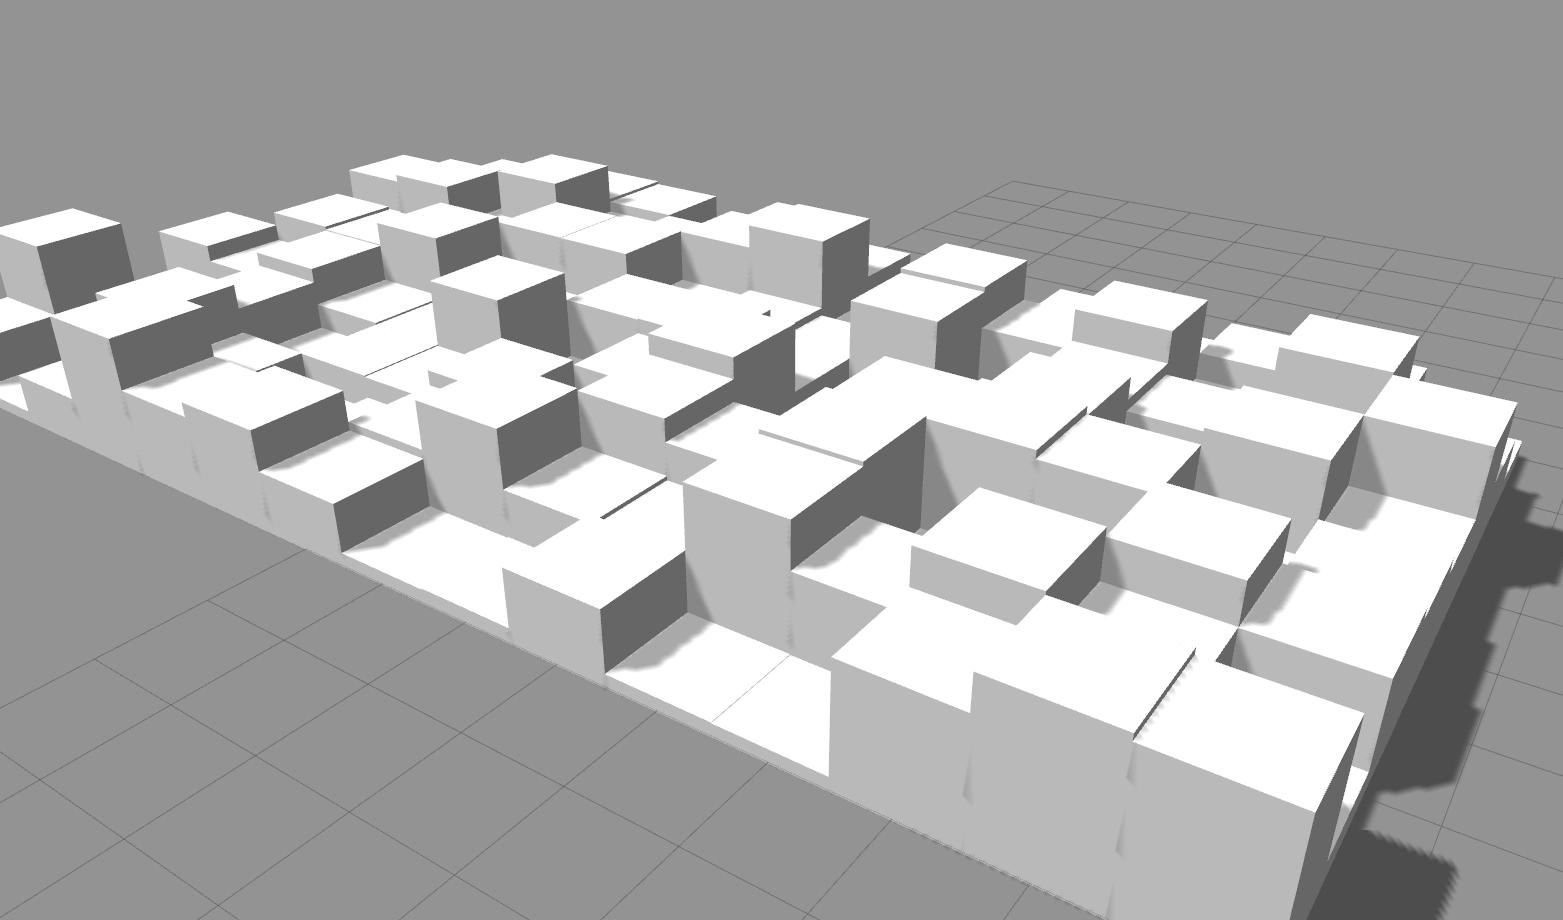
\includegraphics[width=0.8\textwidth]{terrain_1} 
    \caption{T1: 3D-боксы с равномерным распределением высоты}
    \label{fig:terrain_1}
    \end{subfigure}
    \begin{subfigure}{0.33\textwidth}
    \centering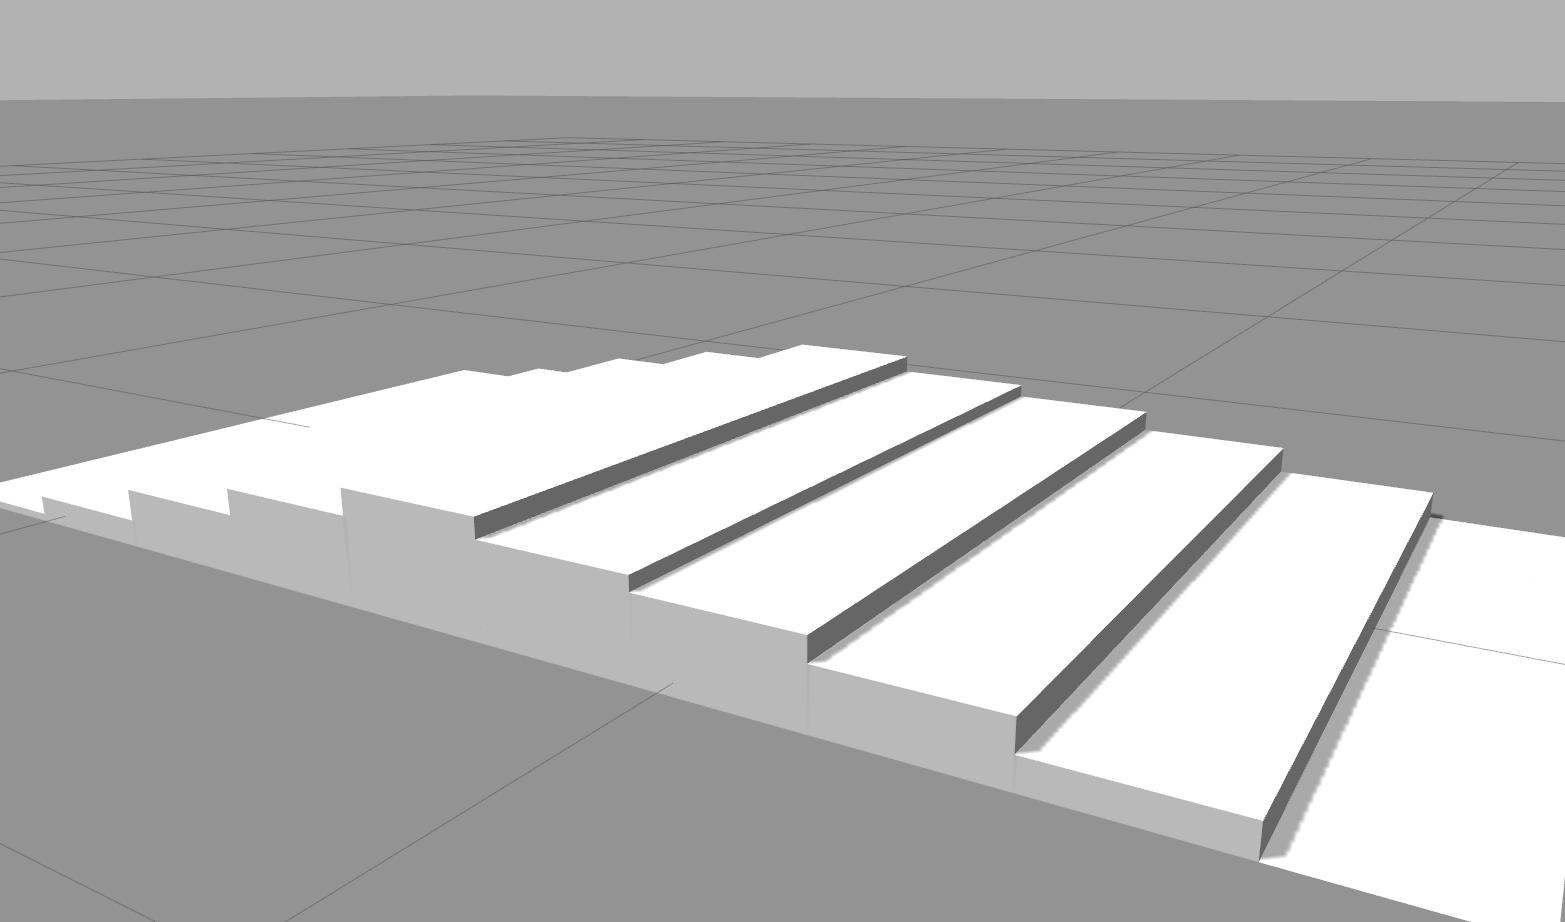
\includegraphics[width=0.8\textwidth]{terrain_2} 
    \caption{T2: 2D-полосы с гауссовой функциональной высотой}
    \label{fig:terrain_2}
    \end{subfigure}
    \begin{subfigure}{0.33\textwidth}
    \centering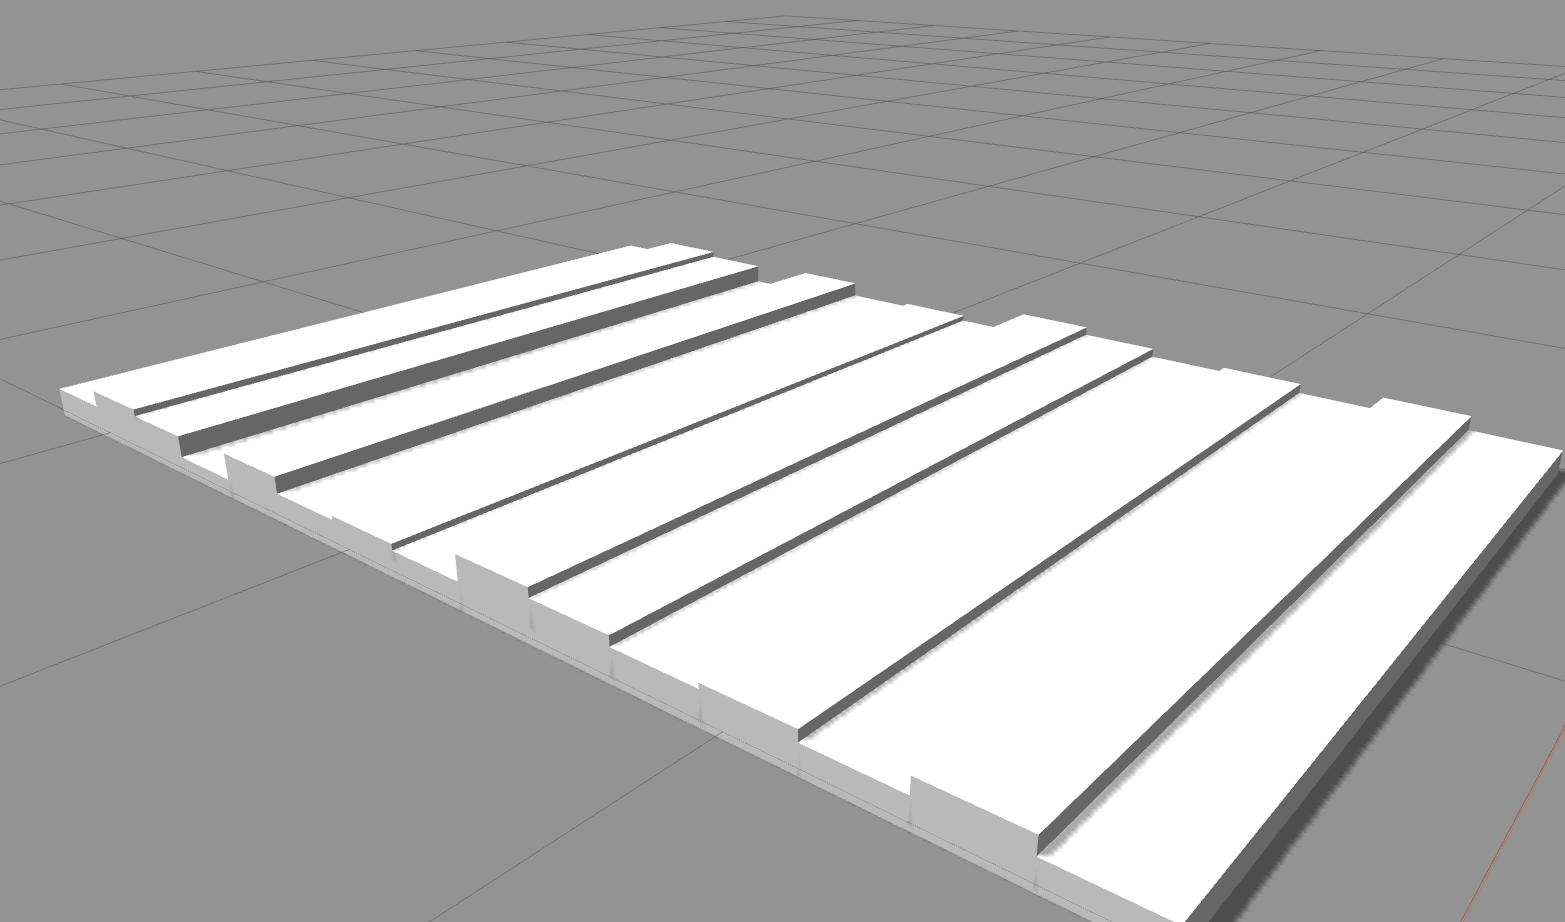
\includegraphics[width=0.8\textwidth]{terrain_3}
    \caption{T3: 2D-полосы с распределением высоты по гауссовой функции)}
    \label{fig:terrain_3}
    \end{subfigure}
     
    \caption{Примеры сгенерированных территорий}
    \label{fig:terrains}
\end{figure}

Геометрическая модель робота представлена в виде трехмерного параллелепипеда. Количество движителей по каждому из бортов обозначается через $\gamma$. Разность фаз между соседними движителями обозначается через  $\alpha$ \pic{fig:best_gen_robot.jpg}.

\begin{figure}[H]
    \centering
    \begin{tikzpicture}
        % Include the image in a node
        \node [above right, inner sep=0] (image) at (0,0)
        {\centering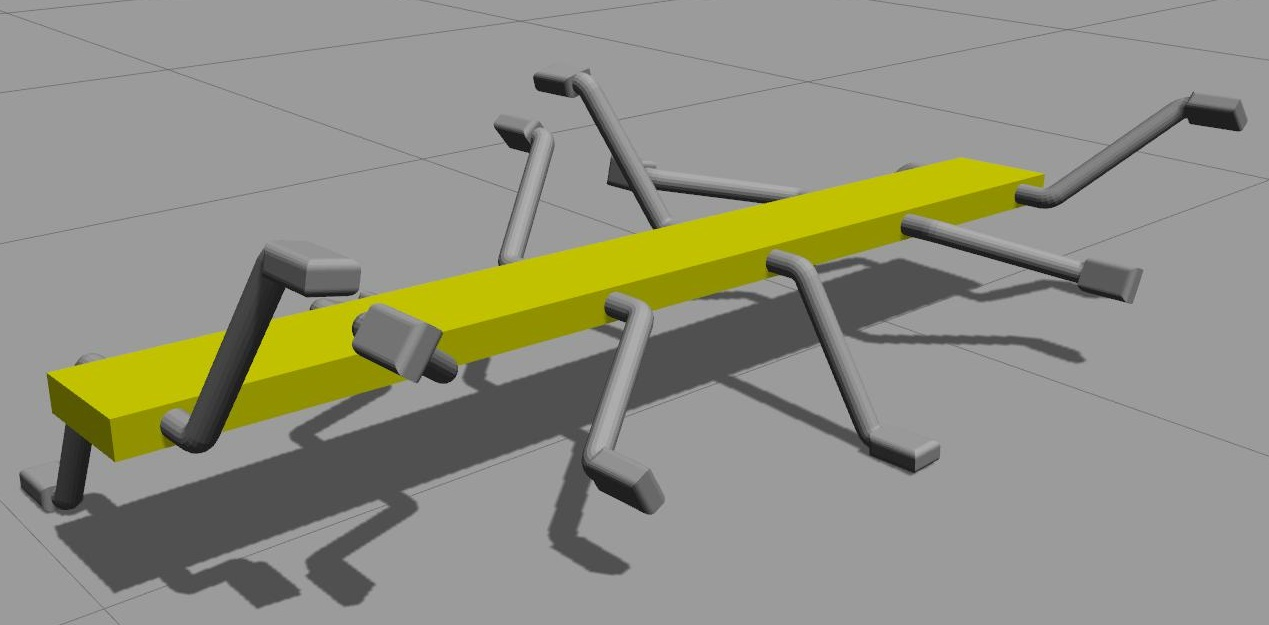
\includegraphics[height=2.7cm,width=1\textwidth,keepaspectratio]{best_gen_robot.jpg}};
        % Create scope with normalized axes
        \begin{scope}[
                x={($ 0.1*(image.south east)$)},
                y={($ 0.1*(image.north west)$)}]
            % Labels
            \draw [green, very thick,
                decorate,
                decoration = {brace,
                        raise=5pt,
                        amplitude=5pt,
                        aspect=0.5}] (1.4,3.6) --  (8.1,6.8)
            node[rounded corners=3pt, pos=0.5,above left =14pt,black,fill=white]{\tiny $(\gamma - 1) h_{\text{leg}}sin(\alpha)$};

            \draw[stealth-, very thick,green] (9.5,7.8) -- (7.8,1.94);
            \draw[stealth-, very thick,green] (1.5,2.8) -- (7,1)
            node[rounded corners=3pt,right,black,fill=white]{\tiny $\gamma = 6$};

            \draw[thin,green] (6.7,4) -- (5.75,9);
            \draw[thin,green] (4.85,3.5) -- (5.75,9);
            \draw[thin,green,stealth-stealth] (6.32,6) arc (-79.2:-99.2:3) node [rounded corners=3pt,below = 2pt,black,fill=white, midway] {\tiny $\alpha$};
        \end{scope}
    \end{tikzpicture}
    \caption{Схема модели робота для генетического алгоритма}
    \label{fig:best_gen_robot.jpg}
\end{figure}

Для решения задачи оптимизации нужно разработать целевую функцию. Поскольку количество ног и длина корпуса имеют прямую зависимость, то задачу формализована следующим образом. Необходимо максимизировать дистанцию, пройденную за фиксированное время, и минимизировать длину робота \eqref{eq:second}. Параметрами индивида являлись $\gamma$ и $\alpha$. Функция оптимизации осуществлялась с помощью мультипликативно-аддитивной свертки.

\begin{eqnarray}
    \label{eq:second}
    F \rightarrow max = \beta \left( {\omega}_{1} \cdot \delta + {\omega}_{2} \cdot L\right) + \\ \nonumber + (1 - \beta) {\delta}^{{\omega}_{1}} {\left( L\right)}^{{\omega}_{2}} \\
\end{eqnarray}
\begin{align}
    L = \frac{1}{(\gamma - 1) h_{\text{leg}}sin(\alpha)}
\end{align}
где $\delta$ пройденная дистанция, $L$ --- упрощенное представление длины тела, $\beta$ адаптивный параметр, ${\omega}_{1,2} \in  [ 0..1 ] $ весовые коэффициенты.

\textit{Описание математической модели}. Здесь и далее движение робота моделировалось с помощью следующей динамической модели. Робот представляет собой механическую систему, состоящую из твердых тел \eqref{eq:newton_euler}. Движение которых описывается дифференциальными уравнениями вида:

\begin{align}
    \label{eq:newton_euler}
    M \dot{\vec{u}} = \vec{g} \\
    M = \begin{bmatrix}
    M_1 & \cdots  & 0 \\
    \vdots  & \ddots  & \vdots  \\ 
    0 & \cdots   & M_n 
    \end{bmatrix},\ M_i = \begin{bmatrix}
    m_i E_{3\times 3} & 0 \\ 
    0 & I_i 
    \end{bmatrix} \\
    \vec{u}_i^{\ T} = \begin{bmatrix}
        \vec{v}_i^{\ T} & \vec{\omega}_i^{\ T}
    \end{bmatrix} \\ 
    \vec{g}^{\ T} = \begin{bmatrix}
        \cdots \  \vec{F}_i^{\ T}, & (\vec{\tau}_i - \vec{\omega}_i \times I_i \vec{\omega}_i)^T\  \cdots 
    \end{bmatrix}
\end{align}
где, $M_i$ --- матрицы, содержащие массово-инерционные характеристики; $m_i$ масса тела; $I_i$ тензор инерции; $\vec{u_i}$ вектор обобщённых скоростей; $E$ --- единичная матрица; $\vec{g}$ вектор обобщённых сил; $\vec{v_i}$ вектор линейной скорости; $\vec{\omega_i}$ --- вектор угловой скорости; $\vec{F_i}$, $\vec{\tau_i}$ силы и моменты сил взаимодействия.

Тела, входящие в систему соединены между собой цилиндрическими шарнирами, которые описываются следующими связями и динамическими ограничениями \eqref{eq:kin_constr}:
\begin{align}
    \label{eq:kin_constr}
    \phi(q_{j_1},\ u_{j_1},\ \cdots,\ q_{j_k},\ u_{j_k},\ t) \geqslant  0 \\
    \vec{q_i}^{\ T} = \begin{bmatrix}
        \vec{x}_i^{\ T} & \vec{Q}_i^{\ T}
    \end{bmatrix} \\
    \dot{\vec{q_i}} = \begin{bmatrix}
    E_{3\times3} & 0\\ 
    0 & G(\vec{q}_i) 
    \end{bmatrix}\vec{u}_i  \\
    \vec{g}_i = \tau_i^T \vec{z}_{i-1} -k_i \dot{\vec{q_i}}
\end{align}
где через $\phi$ обозначена функция связи; $t$ время; $q_{j}$ --- вектор обобщенных координат, включающий в себя координаты центра масс $\vec{x_i}$ и кватернион $\vec{Q_i}$, описывающий ориентацию тела в пространстве; через $G(\vec{q}_i)$ обозначена матрица, вид которой зависит от выбранной системы координат и способа задания ориентации тела; $k$~---~ коэффициент вязкого трения в шарнире.

Контакт ног робота с опорной поверхностью \pic{fig:contact_interaction.png} описывается на базе модели сухого трения и выражается следующими уравнениями \eqref{eq:contact_inter}:


\begin{align}
    \label{eq:contact_inter}
    \phi_u(\vec{q}\ ) \geqslant 0 \\ 
                        \phi_u(\vec{q}\ ) = (\vec{x}_1 + \vec{s}_1 - \vec{x}_2 - \vec{s}_2) \cdot \vec{n} \\
                        \frac{d }{d t}\phi_u(\vec{q}\ ) \approx \begin{bmatrix}
                            \vec{n}^{\ T} & (\vec{s}_1 \times \vec{n})^T & -\vec{n}^{\ T} & (-\vec{s}_2 \times \vec{n})^T
                        \end{bmatrix} \begin{bmatrix}
                            \vec{v}_1\\ 
                        \vec{\omega}_1\\ 
                        \vec{v}_2\\
                        \vec{\omega}_2\\
                        \end{bmatrix} \\
\left\{\begin{matrix*}[l]
\mu f_n \geqslant \sqrt{f_1^2 + f_2^2}\\ 
\left\lVert \vec{v_t}\right\rVert (\mu f_n - \sqrt{f_1^2 + f_2^2}) = 0\\
\dfrac{\vec{f_t}}{\left\lVert \vec{f_t}\right\rVert } = - \dfrac{\vec{v_t}}{\left\lVert \vec{v_t}\right\rVert }
\end{matrix*}\right.
\end{align}
где, $\phi_u(\vec{q})$ --- функция связи; $\mu $ --- коэффициент трения между ногой и опорной поверхностью; $\vec{x}_{1,2},\ \vec{s}_{1,2}$ --- радиус-векторы и орты координатных осей $\vec{t}_{1,2}, \vec{n}$ показаны на рисунке \pic{fig:contact_interaction.png}; $ f_{1,2} $ --- значения сил трения вдоль осей $t_{1,2}$ соответственно.

\begin{figure}[H]
    \centering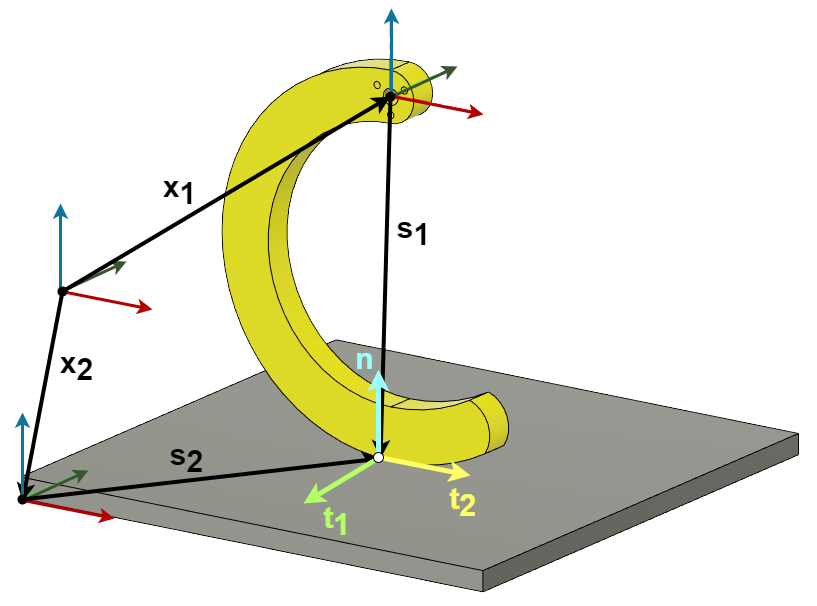
\includegraphics[height=5cm,width=1\textwidth,keepaspectratio]{images/contact_interaction.png}
    \caption{Отображение переменных для модели взаимодействия опорной поверхности и ноги робота}
    \label{fig:contact_interaction.png}
\end{figure}



Численные эксперименты выполнялись в симуляторе Gazebo. В качестве примера видеозапись одного из экспериментов можно посмотреть по ссылке в QR-коде \quad \qrcode[height=1.5cm]{https://youtu.be/DcovvkTZgsg}

Одним из основных результатов исследования, полученных при варьировании значений весовых коэффициентов $\omega$ является зависимость между количеством ног и пройденной дистанцией \pic{fig:box_plot_structural_synthesis.png}, которая показала наличие локального оптимума при количестве ног у робота в диапазоне от 8 до 14. 

\begin{figure}[H]
    \centering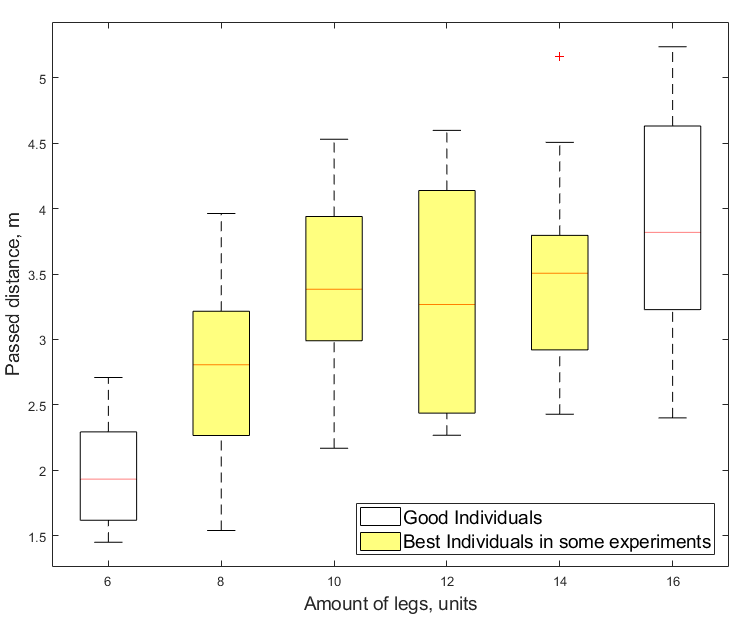
\includegraphics[height=6cm,width=1\textwidth,keepaspectratio]{images/box_plot_structural_synthesis.png}
    \caption{Зависимость между количеством ног и пройденной дистанцией}
    \label{fig:box_plot_structural_synthesis.png}
\end{figure}

\textbf{Вторая задача:} найти оптимальную разность фаз между соседними ногами робота при прямолинейном движении, чтобы средний клиренс был максимально возможным, а колебания корпуса робота --- минимальны. У робота, для которого решалась данная задача ноги двигались синхронно, но в начальный момент времени была возможность выставить произвольную фазу на каждой ноге и она будет сохраняться.

Задача целевой функции --- максимизировать вертикальную координату $Z$ робота и минимизировать среднеквадратичное значение ($RMS$) и среднее стандартное отклонение ($STD$) углов тангажа и крена. Целевая функция учитывает направление движения.

Целевая функция выглядит следующим образом:
\begin{align}
    \label{eq:objective}
    F = \sum\limits_{i=1}^4 \omega_{i} \cdot (\frac{1}{\omega_{z1}Z_{rms}^i - \omega_{z2}Z_{std}^i}  + ( \omega_{p1}\alpha_{rms}^i + \omega_{p2}\alpha_{std}^i) + \nonumber \\\ + (\omega_{r1}\beta_{rms}^i + \omega_{r2}\beta_{std}^i)) \rightarrow min
\end{align}
где $i =\{1,2,3,4\}$ индекс, который определяет направление движения: 1 --- вперед, 2 --- влево, 3 --- вправо, 4 --- вращение; $\alpha, \beta$ значения ориентации по крену и тангажу; $\omega_{i}$ весовой коэффициент для направления движения.

Решение задачи оптимизации проводилось с помощью метода полного перебора. Результатом является оптимальная разность фаз, близкая к 120 градусам.

\textbf{Третья задача:} разработать концепт корпуса робота для максимизации курсовой проходимости, без изменения длины ног робота.

\begin{figure}[H]
    \centering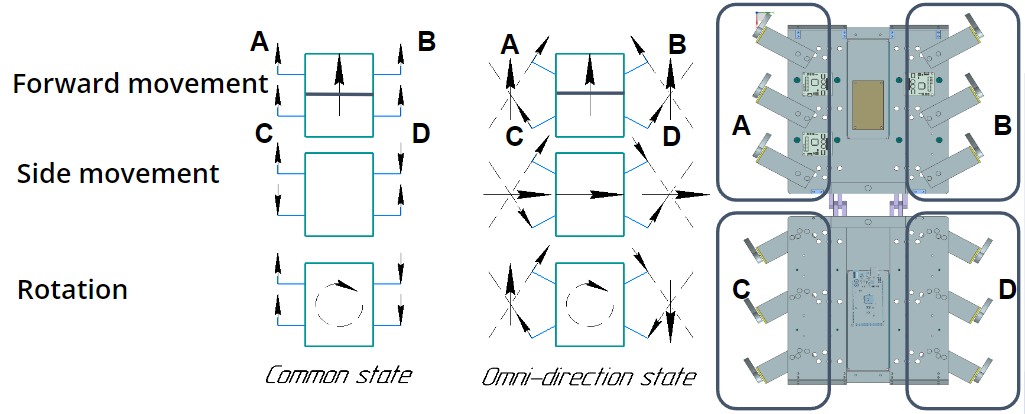
\includegraphics[height=4cm,width=1\textwidth,keepaspectratio]{omni_rot.png}
    \caption{Векторное представление сил в классическом и всенаправленном вариантах робота}
    \label{fig:omnidirection}
\end{figure}



На рисунке \ref{fig:omnidirection} представлена иллюстрация данной концепции: для того, чтобы робот двигался во всех направлениях, необходимо разделить ноги на группы, чтобы получилось 4 группы A-D и сделать так, чтобы угол между корпусом робота и осью вала привода ноги не был равен 90 градусам. 

Стрелка в центре робота --- результирующая всех сил. Если изменить угол оси привода ноги в соответствии с предлагаемой концепцией, к примеру при этапе проектирования или сделать возможность ее изменять во время движения, то возможно получить вектор результирующей силы, представленный на рис. \ref{fig:omnidirection} в центре. Для того, чтобы переместить корпус робота вправо, группы A и D должны вращать ногу в одну сторону, а группы C и B --- в противоположную.

Возможности, полученные с помощью оптимизации конструкции робота можно посмотреть по ссылке в QR-коде \quad \qrcode[height=1.5cm]{https://youtu.be/EQ6oGZVDpoc}

Результатом главы стал метод, который позволяет оптимизировать конструкцию класса многоногих шагающих роботов с цельным или сочленённым корпусом, и цикловыми движителями с одной степенью свободы, управляемые зависимо или независимо друг от друга для решения задачи определения геометрических и физико-механических свойств пройденной поверхности.